%
We will here briefly present the performance of the CELMA-code.
As there are many ways to measure the performance, we will focus on the average internal iterations per output time-step.
As long as the number of processors used is constant, and as long as the underlying solver framework does not change, this number is expected to be more or less constant.
The observed wall-time for the simulations will on the other hand depend on parameters such as the machine the simulations are executed at, if the computational load on the machine on that day was high etc.
Although the \texttt{4.0.0}-version of BOUT++ includes improvements on the memory handling and on the way certain arithmetic operations are operating on the field, the number of iterations presented here should stay roughly the same.

The performance of the $B_0$-scan (without the use of the Boussinesq approximation) is presented in \cref{fig:BoussPerformance}.
%
\begin{figure}[htb]
    \centering
    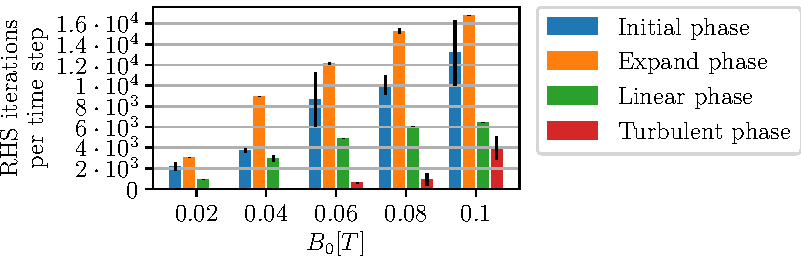
\includegraphics{fig/results/performance/RHSEvalsPerTimeBScan}
    \caption{Performance of the $B$-field scan.}
    \label{fig:BPerformance}
\end{figure}
%
We observe that number of iterations are somewhat high if compared to other codes using the BOUT++ framework.
This is of course dependent of the underlying physical model, which may be stiff under certain conditions \cite{Leveque2007book}.
The two phases responsible for obtaining the steady-state solution requires the most iteration per time-step, despite the fact that the fast dynamics is present only at the beginning of the initialization phase.
Once the perturbation are added to the steady states, the iteration count drops in the linear phase, and drops even further in the turbulent phase.
This is contrary to what is usually observed in turbulence simulations, where the simulation slows down at the onset of turbulence as the solver must resolve a larger specter of eigenmodes.
There may be several reasons for the iteration count in the initialization exceeds that of the turbulent phase, but this has not been investigated in depth in this work.
Instead, we will here present some plausible reasons for the high observed iteration count for the steady state.
It could be that the see-sawing pattern described in \cref{sec:resolution} is limiting the time-step as spurious gradients are being set up between each perpendicular plane.
Next, there may be some numerically fast-traveling waves in the system which might be mitigated by introducing electromagnetic effects \cite{Dudson2015Private}.
The time solver may also be sub-optimized, and it tries to resolve the system at the noise level, or the adaptive time-step controller is frequently choosing time-steps close to a numerical unstable region so that the internal time-step observed comes from the time-step controller trying to find the correct time-step.
In any case, we can see that the number of iterations needed for the next output time-step scales almost linearly with $B_0$ for all phases with exception of the turbulent phase, where the increase in required time-step exceeds a linear scaling.
This scaling is expected as we need to resolve smaller scales at higher magnetic field strengths as $\rho_s$ decreases with $B$.

We can compare our findings of the $B$-scan simulations using the Boussinesq approximation.
This is depicted in \cref{fig:BoussPerformance}.
%
\begin{figure}[htb]
    \centering
    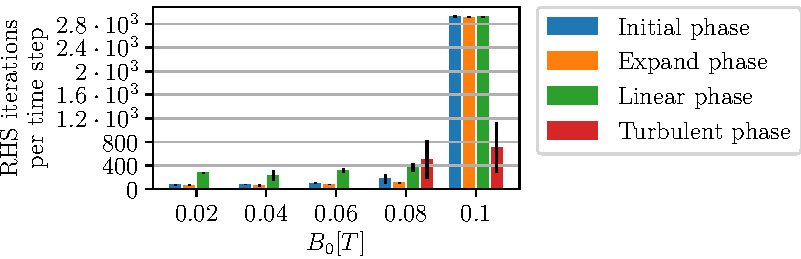
\includegraphics{fig/results/performance/RHSEvalsPerTimeBoussinesqScan}
    \caption{Performance of the $B$-field scan using the Boussinesq approximation.}
    \label{fig:BoussPerformance}
\end{figure}
%
The first thing to note is that the there is up to $90 \%$ reduction of the iteration count in these simulations, with $80\%$ reduction of the iterations of the turbulent phase for $B_0=0.1\T$.
This can indicate that the Boussinesq model is less stiff than the model which do not use the approximation.
We also note that, with exception of $B_0=0.1\T$, the turbulent phase is the most computational demanding in terms of the iteration count.

The iteration count investigation has also been done for the neutral scan, and is shown in \cref{fig:neutPerformance}, and we observe a reduction in the number of iterations for increasing neutral density.
%
\begin{figure}[htb]
    \centering
    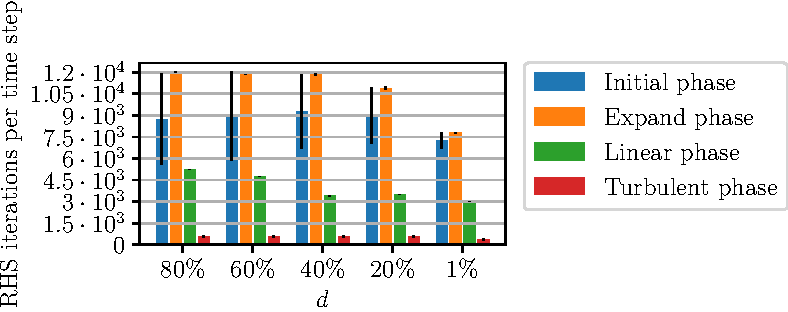
\includegraphics{fig/results/performance/RHSEvalsPerTimeNeutralScan}
    \caption{Performance of the neutral scan using $B_0=0.06\T$.}
    \label{fig:neutPerformance}
\end{figure}
%
This can be understood in terms of the increased collisionality as the neutral collisions adds dissipations to the system.

It is also interesting to investigate what kind of numerical operation which contributes most to the computation time.
This is presented for the $B_0 = 0.06\T$ with $n_n=0$ in \cref{fig:BPct}, and for $B_0 = 0.06\T$ with $n_n=1.5\cdot10^{19}\m^{-3}$ in \cref{fig:neutPct}.
%
\begin{figure}[htb]
    \centering
    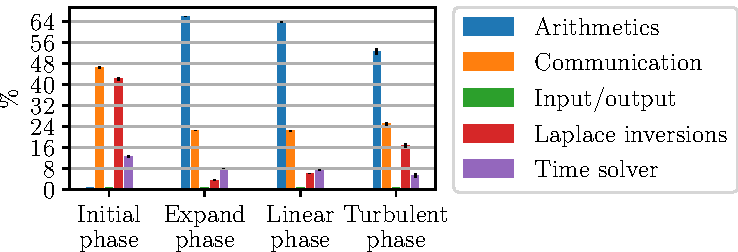
\includegraphics{fig/results/performance/PercentagesBScanB00_06}
    \caption{The time spent on of each computational task in per cent for $B_0=0.06\T$.}
    \label{fig:BPct}
\end{figure}
%
%
\begin{figure}[htb]
    \centering
    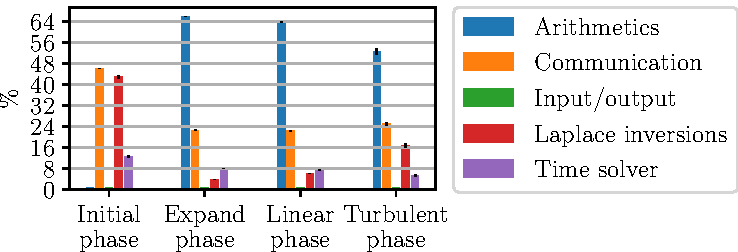
\includegraphics{fig/results/performance/PercentagesNeutralScanB00_06Nn1_5e+19}
    \caption{The time spent on of each computational task in per cent for $B_0=0.06\T$ with an ionization degree of $d=40\%$.}
    \label{fig:neutPct}
\end{figure}
%
%
\begin{figure}[h!]
    \centering
    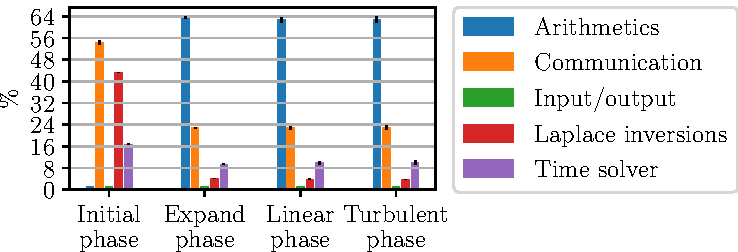
\includegraphics{fig/results/performance/PercentagesBousScanB00_08}
    \caption{The time spent on of each computational task in per cent for $B_0=0.08\T$ using the Boussinesq approximation.}
    \label{fig:BoussPct}
\end{figure}
%
The figures are almost identical in terms of the computational work distribution for all phases.
Although the added collisionality may reduce the iteration count, there is no obvious reason for why the computational work distribution should change.
In the neutral simulations only the value of $\nu_{en}$ is changed.
Although $\nu_{en}=0$, the neutral collision terms are still being calculated in the code, which means that the time spent on doing arithmetic operations on fields (like $+$, $-$ etc.) is not expected to change.
From \cref{fig:BPct,fig:neutPct} we can see that most of the communication is spent at arithmetic operations, followed by communication of the domain boundary between the different processors%
\footnote{Parallelization in the simulations is done by a domain split in the $\rho$ and $z$ direction with domain boundary communication using \texttt{Message Parsing Interface} included in the BOUT++ framework.}%
.
The Laplace inversions done with the iterative Naulin solver seems to be important only in the turbulence phase.
It is found that the solver uses between $3-10$ iteration per time-step in this phase.

We can compare this workload with the ones found for the Boussinesq approximation for $B_0=0.08\T$, shown in \cref{fig:BoussPct}.
The work load is still dominated by the arithmetics and communications.
However, there is a decrease in time spent in the Laplace solver, which can be explained by the fact that only one inversion is needed per iteration.
This may also contribute to the decrease of the iteration count presented above.
